\documentclass[colorlinks,11pt,a4paper,normalphoto,withhyper,ragged2e]{altareport}


%%%%%%%%%%%%%%%%%%%%%%%%%%%%%%%%%%%%%%%%%%%%%%%%%%%%%%%%%%%%%%%%%%%%%%%%%%%%%%%%%%%%%%%%%%%%%%%%%%%%%%%%%%%%%%%%%%%%%%%%%%%%%%%%%%%%%%%%%%%%%%%%%%%%%%%%%%%%%%%%%%%%%%%%%%%%
%%%%%%%%%% DEFAULT PACKAGES & SETTINGS %%%%%%%%%%
\usepackage{setspace} %1.5 line spacing
\usepackage{notoccite} %% Citation numbering
\usepackage{lscape} %% Landscape table
\usepackage{caption} %% Adds a newline in the table caption
\usepackage[rgb]{xcolor}

%% The paracol package lets you typeset columns of text in parallel
\usepackage{paracol}
\usepackage[none]{hyphenat}

%%% Document/Theme Fonts, Space and Text Settings
\usepackage{fontspec}
\setmainfont{Roboto Slab}
\setsansfont{Lato}
\renewcommand{\familydefault}{\sfdefault}
\captionsetup{font=footnotesize} % Make Captions a sensible size
\setlength{\intextsep}{4pt} % Set defualt spacing around floats
% \captionsetup{aboveskip=5pt, belowskip=5pt} % Reduce space around captions
\geometry{left=1.25cm,right=1.25cm,top=2.5cm,bottom=2.5cm,columnsep=8mm} % Change the page layout
\setstretch{1.5}   % 1.5 line spacing
\definecolor{CommentGreen}{HTML}{228B22}
\justifying

%% Math Env Text Settings
\usepackage{mathtools}
\usepackage{unicode-math}
\setmathfont{XITS Math}
\usepackage{amsmath}
\usepackage{bm}
\everymath=\expandafter{\the\everymath\displaystyle}
%%%%%%%%%%%%%%%%%%%%%%%%%%%%%%%%%%%%%%%%%%%%%%%%%%%%%%%%%%%%%%%%%%%%%%%%%%%%%%%%%%%%%%%%%%%%%%%%%%%%%%%%%%%%%%%%%%%%%%%%%%%%%%%%%%%%%%%%%%%%%%%%%%%%%%%%%%%%%%%%%%%%%%%%%%%%


%%%%%%%%%%%%%%%%%%%%%%%%%%%%%%%%%%%%%%%%%%%%%%%%%%%%%%%%%%%%%%%%%%%%%%%%%%%%%%%%%%%%%%%%%%%%%%%%%%%%%%%%%%%%%%%%%%%%%%%%%%%%%%%%%%%%%%%%%%%%%%%%%%%%%%%%%%%%%%%%%%%%%%%%%%%%
%%%%%%%%%% DOCUMENT SPECIFIC PACKAGES AND SETTINGS %%%%%%%%%%

\SetTheme{UNIBS}






%%%%%%%%%%%%%%%%%%%%%%%%%%%%%%%%%%%%%%%%%%%%%%%%%%%%%%%%%%%%%%%%%%%%%%%%%%%%%%%%%%%%%%%%%%%%%%%%%%%%%%%%%%%%%%%%%%%%%%%%%%%%%%%%%%%%%%%%%%%%%%%%%%%%%%%%%%%%%%%%%%%%%%%%%%%%
%%%%%%%%%% TITLE PAGE INFO %%%%%%%%%%
\ReportTitle{Remote Sensing Data Acquisition}
\SubTitle{Beam Four Exercise - 28/08/2023}
\Author{Andrew Simon Wilson}
\ReportDate{\today}
\FacultyOrLocation{EMIMEO Programme}
\ModCoord{Prof. Daniele Modotto}

%%%%%%%%%%%%%%%%%%%%%%%%%%%%%%%%%%%%%%%%%%%%%%%%%%%%%%%%%%%%%%%%%%%%%%%%%%%%%%%%%%%%%%%%%%%%%%%%%%%%%%%%%%%%%%%%%%%%%%%%%%%%%%%%%%%%%%%%%%%%%%%%%%%%%%%%%%%%%%%%%%%%%%%%%%%%


%%%%%%%%%%%%%%%%%%%%%%%%%%%%%%%%%%%%%%%%%%%%%%%%%%%%%%%%%%%%%%%%%%%%%%%%%%%%%%%%%%%%%%%%%%%%%%%%%%%%%%%%%%%%%%%%%%%%%%%%%%%%%%%%%%%%%%%%%%%%%%%%%%%%%%%%%%%%%%%%%%%%%%%%%%%%
%%%%%%%%%% STAGING AREA %%%%%%%%%%
\usepackage{relsize}
\usepackage{subcaption}






%%%%%%%%%% DOCUMENT CONTENT %%%%%%%%%%
\begin{document}

	\MakeReportTitlePage
	
	
	%%%%% CONTENTS %%%%%
	\pagenumbering{roman} % Start roman numbering
	\setcounter{page}{1}
	
	
%	%%%%%%%%%% YOUR NAME, PROFESSION, PORTRAIT, CONTACT INFO, SOCIAL MEDIA ETC. %%%%%%%%%%
%	\name{Andrew Simon Wilson, BEng}
%	\tagline{Post-graduate Master's Student - EMIMEO Programme}
%	
%	\personalinfo{
%		\email{andrew.wilson@protonmail.com}
%		\linkedin{andrew-simon-wilson} 
%		\github{AS-Wilson}
%		\phone{+44 7930 560 383}
%	}
%	
%	%% You can add multiple photos on the left or right
%	% \photoR{3cm}{Images/a-wilson-potrait.jpg}
%	% \photoL{3cm}{Yacht_High,Suitcase_High}
%	
%	\section*{Author Details}
%	\makeauthordetails
%	
%	%% Table of contents print level -1: part, 0: chapter, 1: section, 2:sub-section, 3:sub-sub-section, etc.
%	\setcounter{tocdepth}{2} 
%	\tableofcontents %% Prints a list of all sections based on the above command
%	%\listoffigures %% Prints a list of all figures in the report
%	%\listoftables %% Prints a list of all tables in the report
%	
%	
%	
%	
%	%%%%%%%%%%% DOCUMENT CONTENT BEGINS HERE %%%%%%%%%%
%	%
%	%%%%%% INTRO %%%%%
%	%\section*{Explanation and Introduction of this Document}
%	%I wrote this document for the students studying Quantum Technologies to have a nice set of notes, and correct reference code and graphs for the module. I hope that it is sufficient for this task and it helps all of your studies. \linebreak
%	%I spent have spent a lot of time developing the template used to make this {\LaTeX} document, I want others to benefit from this work so the source code for this template is available on GitHub \cite{latex_template_github}.
%	
%	
%	\newpage
	\pagenumbering{arabic} % Start document numbering - roman numbering




	\section{Introduction}
		The exercise involves the study and verification of various lens equations, the set-ups of each task are shown in a simple graphical form below in Figures \ref{fig:lens_single} and \ref{fig:lens_compound}. My general approach is to choose any required parameters, theoretically calculate expected values for these parameters, and then verify that these results are true using the Beam Four software, explaining any discrepancies if necessary. \linebreak
		The only parameters of the system which remain constant for the two exercises is the refractive index of the lens material, $n=2.2$, and the focal length of my first bi-convex lens. \linebreak
		
		
		\tikzset{>=latex}
\usetikzlibrary{decorations.markings, calc}

% New Command
%% Middle Line Label
\newcommand{\midlabelline}[3]{
	\node (midlabel) at ($ (#1)!.5!(#2) $) {#3};
	\draw[<-] (#1) --  (midlabel);
	\draw[->] (midlabel) -- (#2);
}
%% Point
\newcommand{\point}[3]{
	\draw[fill=black] (#1) circle (1pt) node[#3] {#2};
}

% Styles
%% Arrow in the Middle
\tikzset{arrow inside/.style = {postaction=decorate,decoration={markings,mark=at position 0.52 with \arrow{stealth}}}}

% Define Color
\definecolor{glass}{cmyk}{0.2,0,0,0}
		
		\begin{figure}[h]
			\centering
%			\hfill
			\begin{subfigure}{0.47\linewidth}
				\centering
				\begin{tikzpicture}[scale=0.35]
	% Grid
%		\draw[help lines] (-3,-3) grid (6,6);
	
	% Lens		
	\path[fill=glass, draw=black, line width = 0.6] (0,-2.5) .. controls (-0.4,0) .. (0,2.75) .. controls (0.4,0) .. (0,-2.5);
	
	% Axis
	\draw[dashed, black!60] (0,-3) -- (0,3);
	\draw[dashed, black!60] (-8.5,0) -- (8.5,0);
	
	% Ray
	\draw[red, line width = 0.6, arrow inside] (-7,0) -- (-0.4,0.7);	
	\draw[red, line width = 0.6] (-0.4,0.7) -- (0.4,0.7);
	\draw[red, line width = 0.6, arrow inside] (0.4,0.7) -- (7,0);
	
	% Refractive index label
	\draw[black!60, <-] (0.2,1.5) -- (2,2.5) node[right] {\tiny Refractive Index, $n=2.2$, Radius, $R_1$};
	
	%Points
	\draw[fill=red] (-7,0) circle (1pt) node[below] {$S$};
	\draw[fill=red] (7,0) circle (1pt) node[below] {$P$};
	
	% Distances
	\midlabelline{-7,-1.5}{0,-1.5}{$s_o$}
	\midlabelline{0,-1.5}{7,-1.5}{$s_i$}
\end{tikzpicture} 
				\caption{\centering\footnotesize The diagram of a single bi-convex lens set-up with relevant parameters shown.}
				\label{fig:lens_single}
			\end{subfigure}
			\hfill
			\begin{subfigure}{0.47\linewidth}
				\centering
				\begin{tikzpicture}[scale=0.35]
	% Grid
	%		\draw[help lines] (-3,-3) grid (6,6);
	
	% Lens One
	\path[fill=glass, draw=black, line width = 0.6] (0,-2.5) .. controls (-0.4,0) .. (0,2.75) .. controls (0.4,0) .. (0,-2.5);
	
	% Lens Two
	\path[fill=glass, draw=black, line width = 0.6] (3.5,-2.5) .. controls (3.1,0) .. (3.5,2.75) .. controls (3.9,0) .. (3.5,-2.5);

	
	% Axis
	\draw[dashed, black!60] (0,-3) -- (0,3);
	\draw[dashed, black!60] (-8.5,0) -- (12.5,0);
	\draw[dashed, black!60] (3.5,-3) -- (3.5,3);
	
	% Ray
	\draw[red, line width = 0.6, arrow inside] (-7,0) -- (-0.4,0.7);	
	\draw[red, line width = 0.6] (-0.4,0.7) -- (3.8,0.7);
	\draw[red, line width = 0.6, arrow inside] (3.8,0.7) -- (10,0);
	
	% Refractive index label
	\draw[black!60, <-] (0.2,1.5) -- (2,4.5) node[right,align=center] {\tiny Refractive Index, $n=2.2$, Focal Length, $f_1$};
	\draw[black!60, <-] (3.7,1.5) -- (5,2.5) node[right,align=center] {\tiny Refractive Index, $n=2.2$, Focal Length, $f_2$};
	
	%Points
	\draw[fill=red] (-7,0) circle (1pt) node[below] {$S$};
	\draw[fill=red] (10,0) circle (1pt) node[below] {$P$};
	
	% Distances
	\midlabelline{-7,-1.5}{0,-1.5}{$s_o$}
	\midlabelline{0,-1.5}{3.5,-1.5}{$d$}
	\midlabelline{3.5,-1.5}{10,-1.5}{$s_i$}
\end{tikzpicture}
				\caption{\centering\footnotesize The diagram of a compound bi-convex lens set-up with relevant parameters shown.}
				\label{fig:lens_compound}
			\end{subfigure}
%			\hfill
		\end{figure}
		
		
		
		
	\section{Task One}
		Firstly, the Thin Lens formula, as per the provided assignment materials, is shown in Eq. \ref{eqn:thin_lens}, with the values corresponding to those found in figure \ref{fig:lens_single}. Additionally, the Lensmakers' formula, also from the provided assignment materials, is shown below in Eq. \ref{eqn:lens_makers}. It is take by convention that the radii of the lens surfaces are: $R_1>0$ and $R_2<0$. \linebreak
		
		\columnratio{0.4}
		\begin{paracol}{2}
			\begin{equation}
				\frac{1}{f} = \frac{1}{s_o} + \frac{1}{s_i}
			\end{equation}\label{eqn:thin_lens}
			\begin{equation}
				\frac{1}{f} = (n-1) \left( \frac{1}{R_1} - \frac{1}{R_2} \right)
			\end{equation}\label{eqn:lens_makers}
			
			\switchcolumn
			
			With the given refractive index, $n=2.2$, I choose to calculate for a focal length of $f=7cm$ (as this complies to $4cm \leq f \leq 10cm$). I then calculated the radii of the bi-convex lens, with the desire to make $R_1=-R_2$ for simplicity. This gave me the value of $16.8cm$ for the radii (a curvature value in Beam Four of $\approx 0.0595$). \linebreak
			I then set about creating the system in Beam Four with the obtained values, Beam Four does not use units so I will refer to the values as $1,7,0.4, \dots \text{ } u$.
		\end{paracol}
		
		Now if the incoming beams are collimated, or focused to the lens can be verified as correct as long as it focus' such a beam to the focal length, $7u$ in Beam Four or $7cm$ in my chosen parameters. I created the .opt and .ray files for the system and its two variants collimated beams from the left and collimated beams from the right. I also set the $x$ and $z$ goals of the system for use with the "AutoAdjust" function to get more accurate values. \linebreak
		The resulting system is shown below in Figures \ref{fig:t1_l2r} and \ref{fig:t2_r2l}, the achieved focal length is within $0.1u$ ($ \equiv 1mm$) for all rays. There is some distortion due to the height at which the rays enters the lens, this is a normal and known phenomena. \linebreak
		
		
		\begin{figure}[h]
			\centering
			\begin{subfigure}{0.47\linewidth}
				\centering
				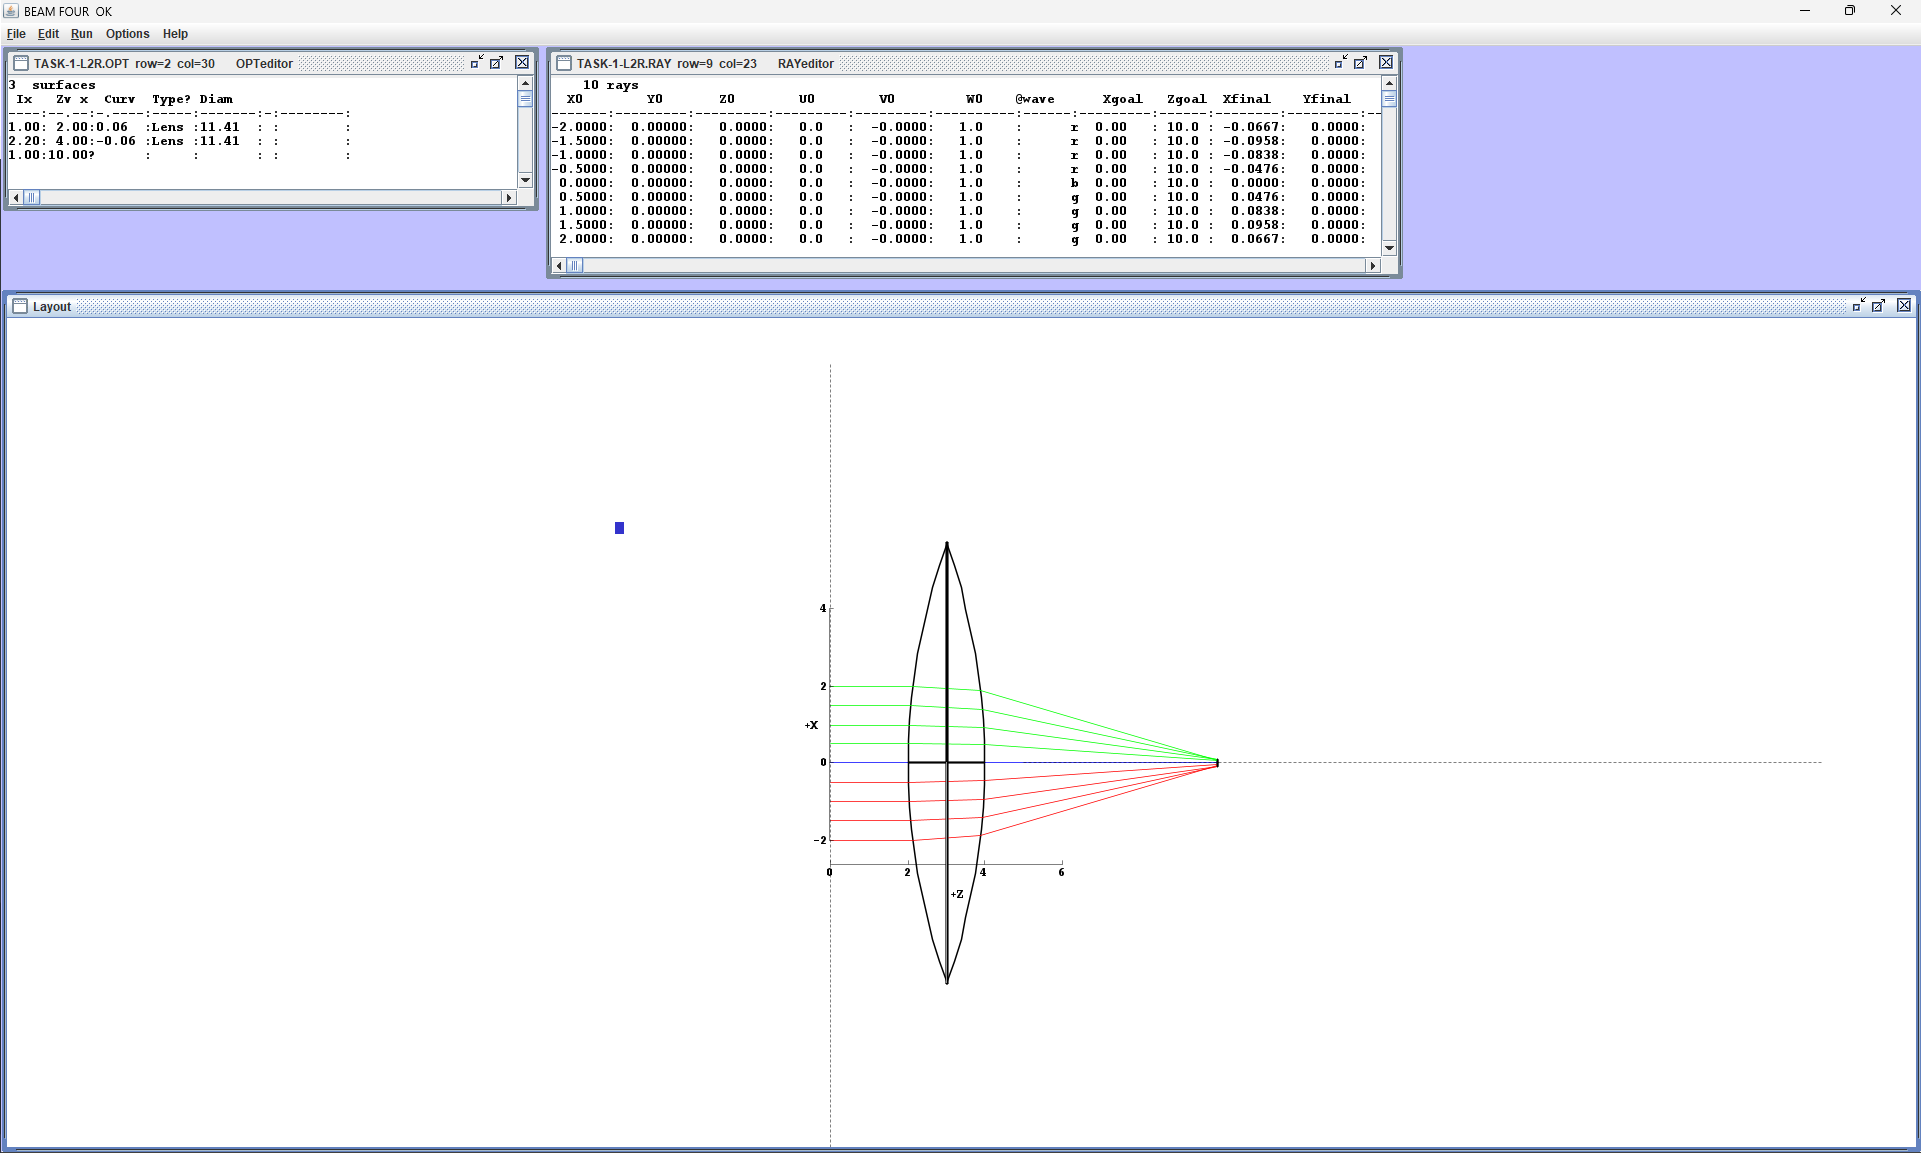
\includegraphics[width=\linewidth]{Images/T1-L2R-Full-Window.png}
				\caption{\centering\footnotesize The beams traveling from left to right, with the relevant system parameters and final values shown.}
				\label{fig:t1_l2r}
			\end{subfigure}
			\hfill
			\begin{subfigure}{0.47\linewidth}
				\centering
				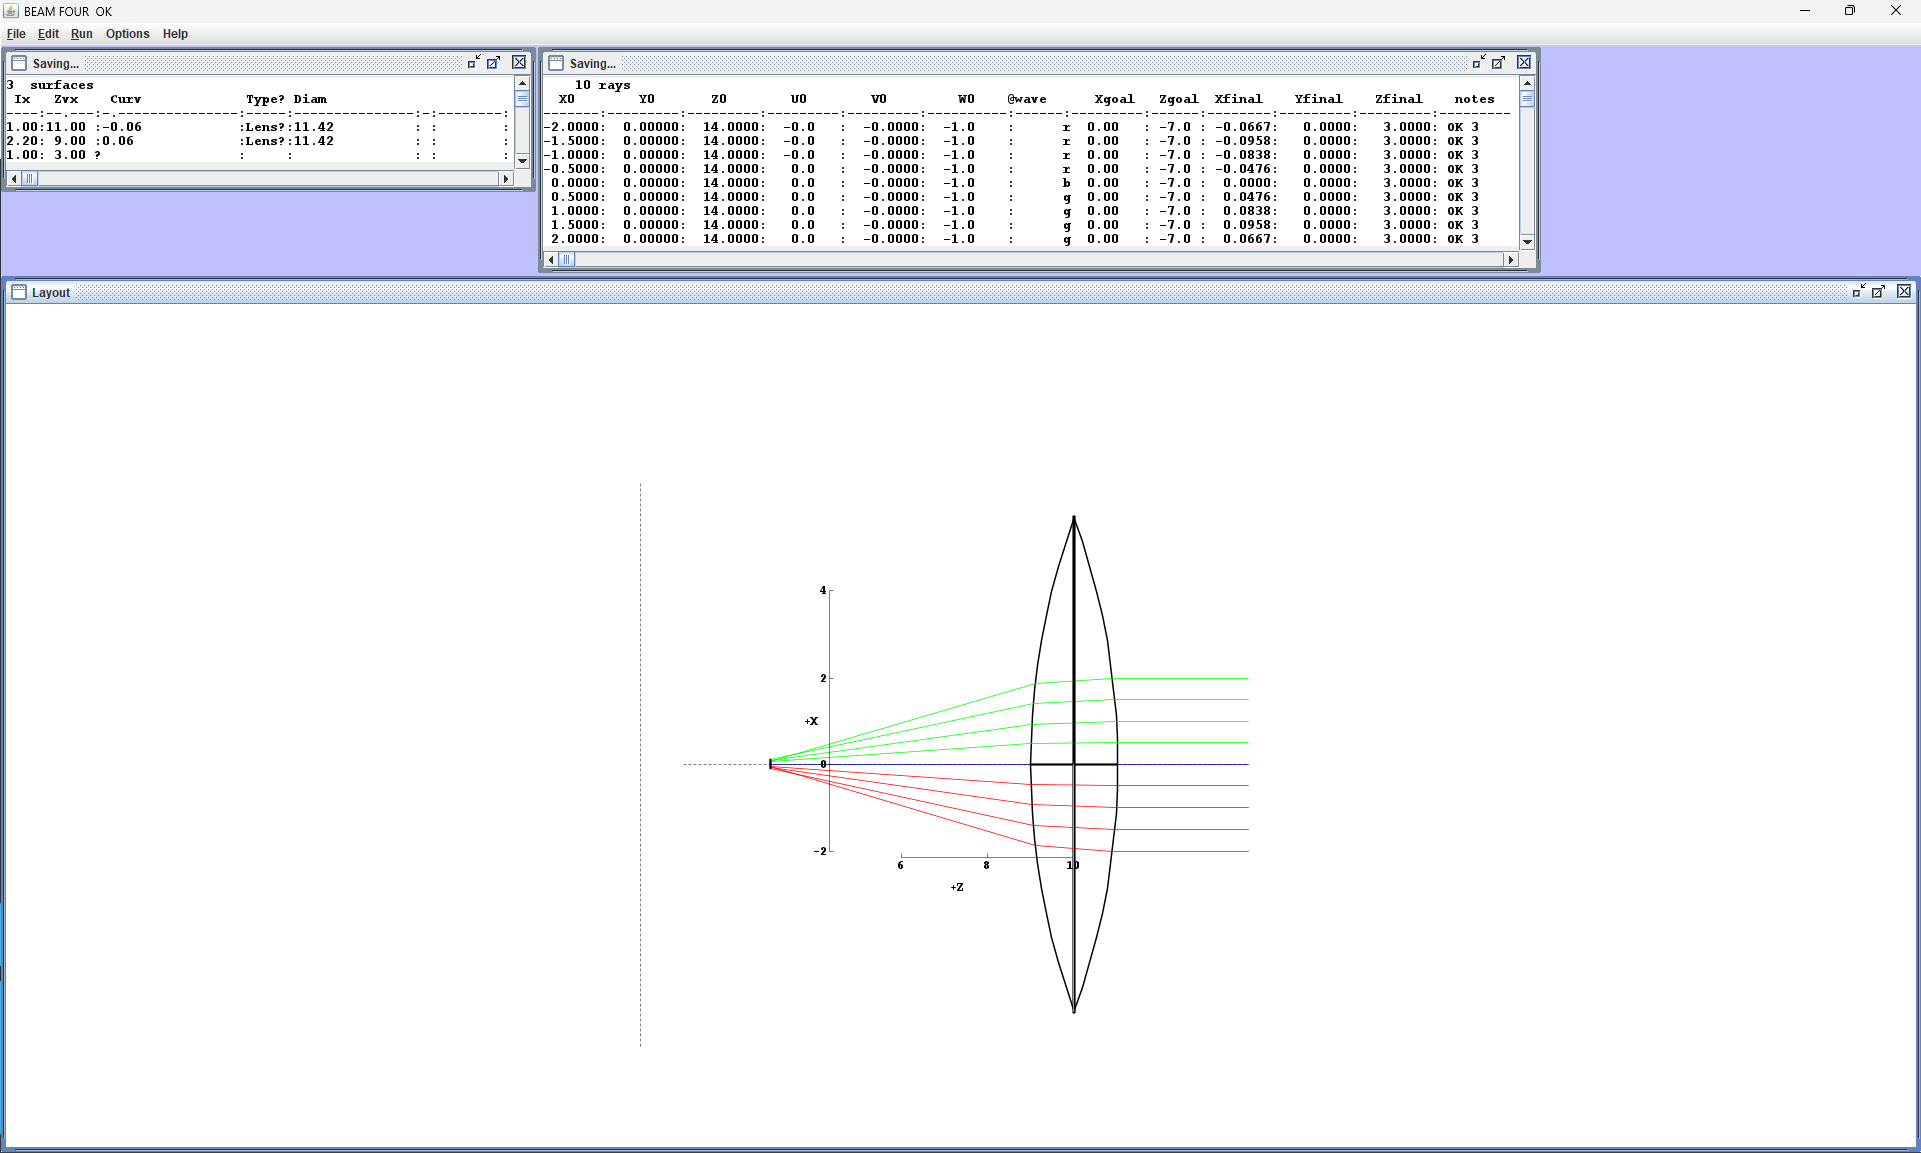
\includegraphics[width=\linewidth]{Images/T1-R2L-Full-Window.png}
				\caption{\centering\footnotesize The beams traveling from right to left, with the relevant system parameters and final values shown.}
				\label{fig:t2_r2l}
			\end{subfigure}
		\end{figure}
		
		Now onto the second task... \linebreak
		
		
		
		
	\section{Task Two}
		\columnratio{0.75}
		\begin{paracol}{2}
			The second task is to confirm the Compound Lens equation (shown in Eq. \ref{eqn:compound_lens}), using at least two different values for parameter $d$, the distance between lens'. Both lens must conform to the limits set out in Task One and have different focal values. As such, I reused the lens from the first task, and calculated/simulated a new lens with a focal length, $f_2=8cm$ (this gives a curvature value in Beam Four of $\approx 0.0521$). \linebreak
			
		\switchcolumn
		
		\begin{equation}
			\mathlarger{\mathlarger{s_i = \frac{f_2 \ d \ \frac{f_1 f_2 s_o}{s_0 - f_1}}{d - f_2 \ \frac{f_1 s_o}{s_o - f_1}}}}
		\end{equation}\label{eqn:compound_lens}
		
		\end{paracol}
		
		I then decided upon an object distance (rays diverging from this point) of $s_0 = 10cm$ ($s_0 = 10u$) from the first lens, and a distance between lens' of $d=10cm$ ($d = 10u$), this should mean that the final focus point of the object, according to the compound lens formula, would be $s_1 \approx 5cm$ ($s_1 = 5u$) from the second lens. I created the system in Beam Four and confirmed that the focus point of the rays is, again, within $0.06u$ ($0.6mm$) of the desired. In beam four this places the focus point of the rays at $\approx 31u$ using the chosen parameters and the compound lens equation. The final values and system is shown in Figure \ref{fig:t2a}: \linebreak
		
		\begin{figure}[h]
			\centering
			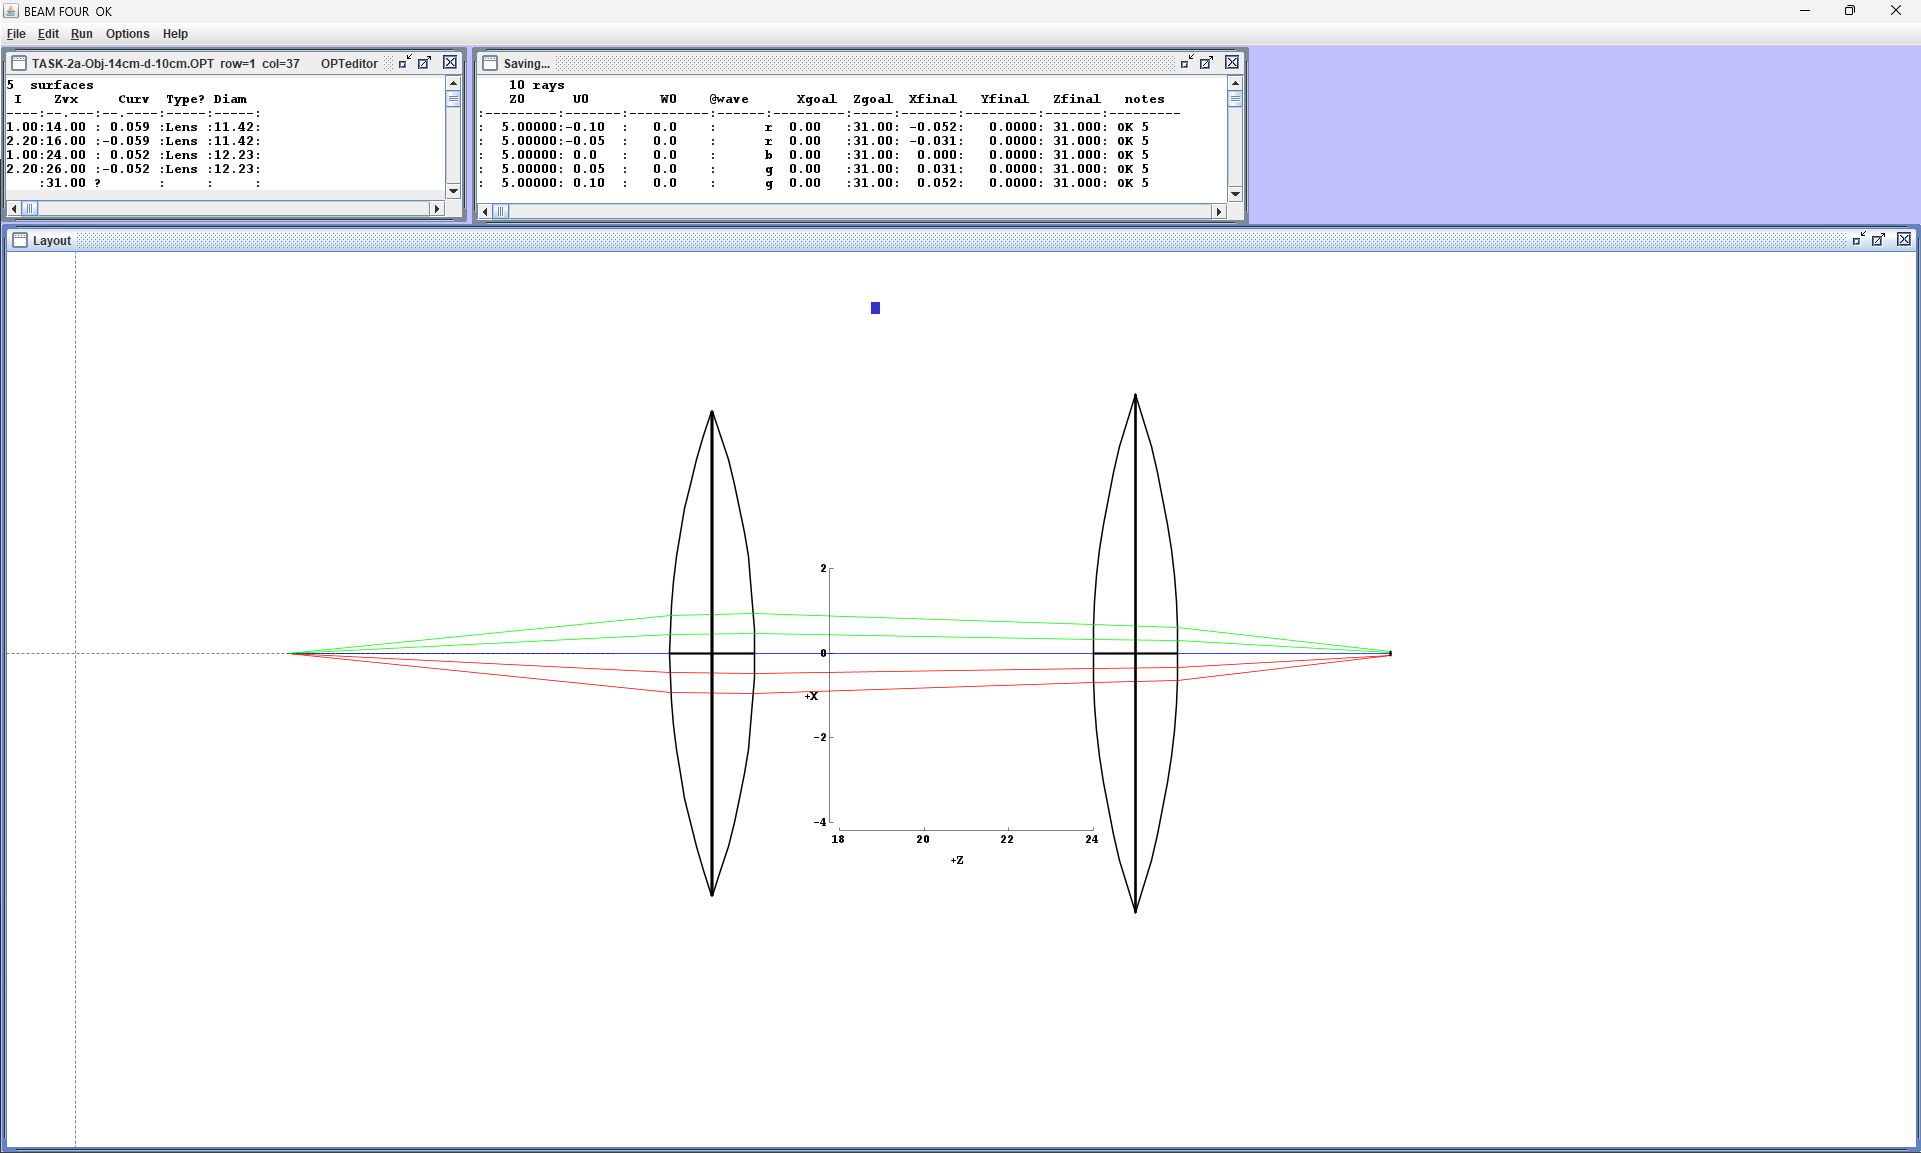
\includegraphics[width=0.75\linewidth]{Images/T2a-obj-10cm-d-10cm-Full-Window.png}
			\caption{\centering\footnotesize The system and beams with the relevant system parameters and final values shown.}
			\label{fig:t2a}
		\end{figure}
		
		\pagebreak
		 
		Then to further confirm the formula, and as per the task request, the distance between lens was changed to $d=4cm$, following the same procedure as before this gives a focus point value of $s_1 \approx 5.66cm$ ($s_1 \approx 5.66u$), In beam four this places the focus point of the rays at $\approx 25.66u$. I created the system in Beam Four and confirmed that the focus point of the rays is, again, within $0.02u$ ($0.2mm$) of the desired, this is shown in Figure \ref{fig:t2b} below: \linebreak
		
		\begin{figure}[h]
			\centering
			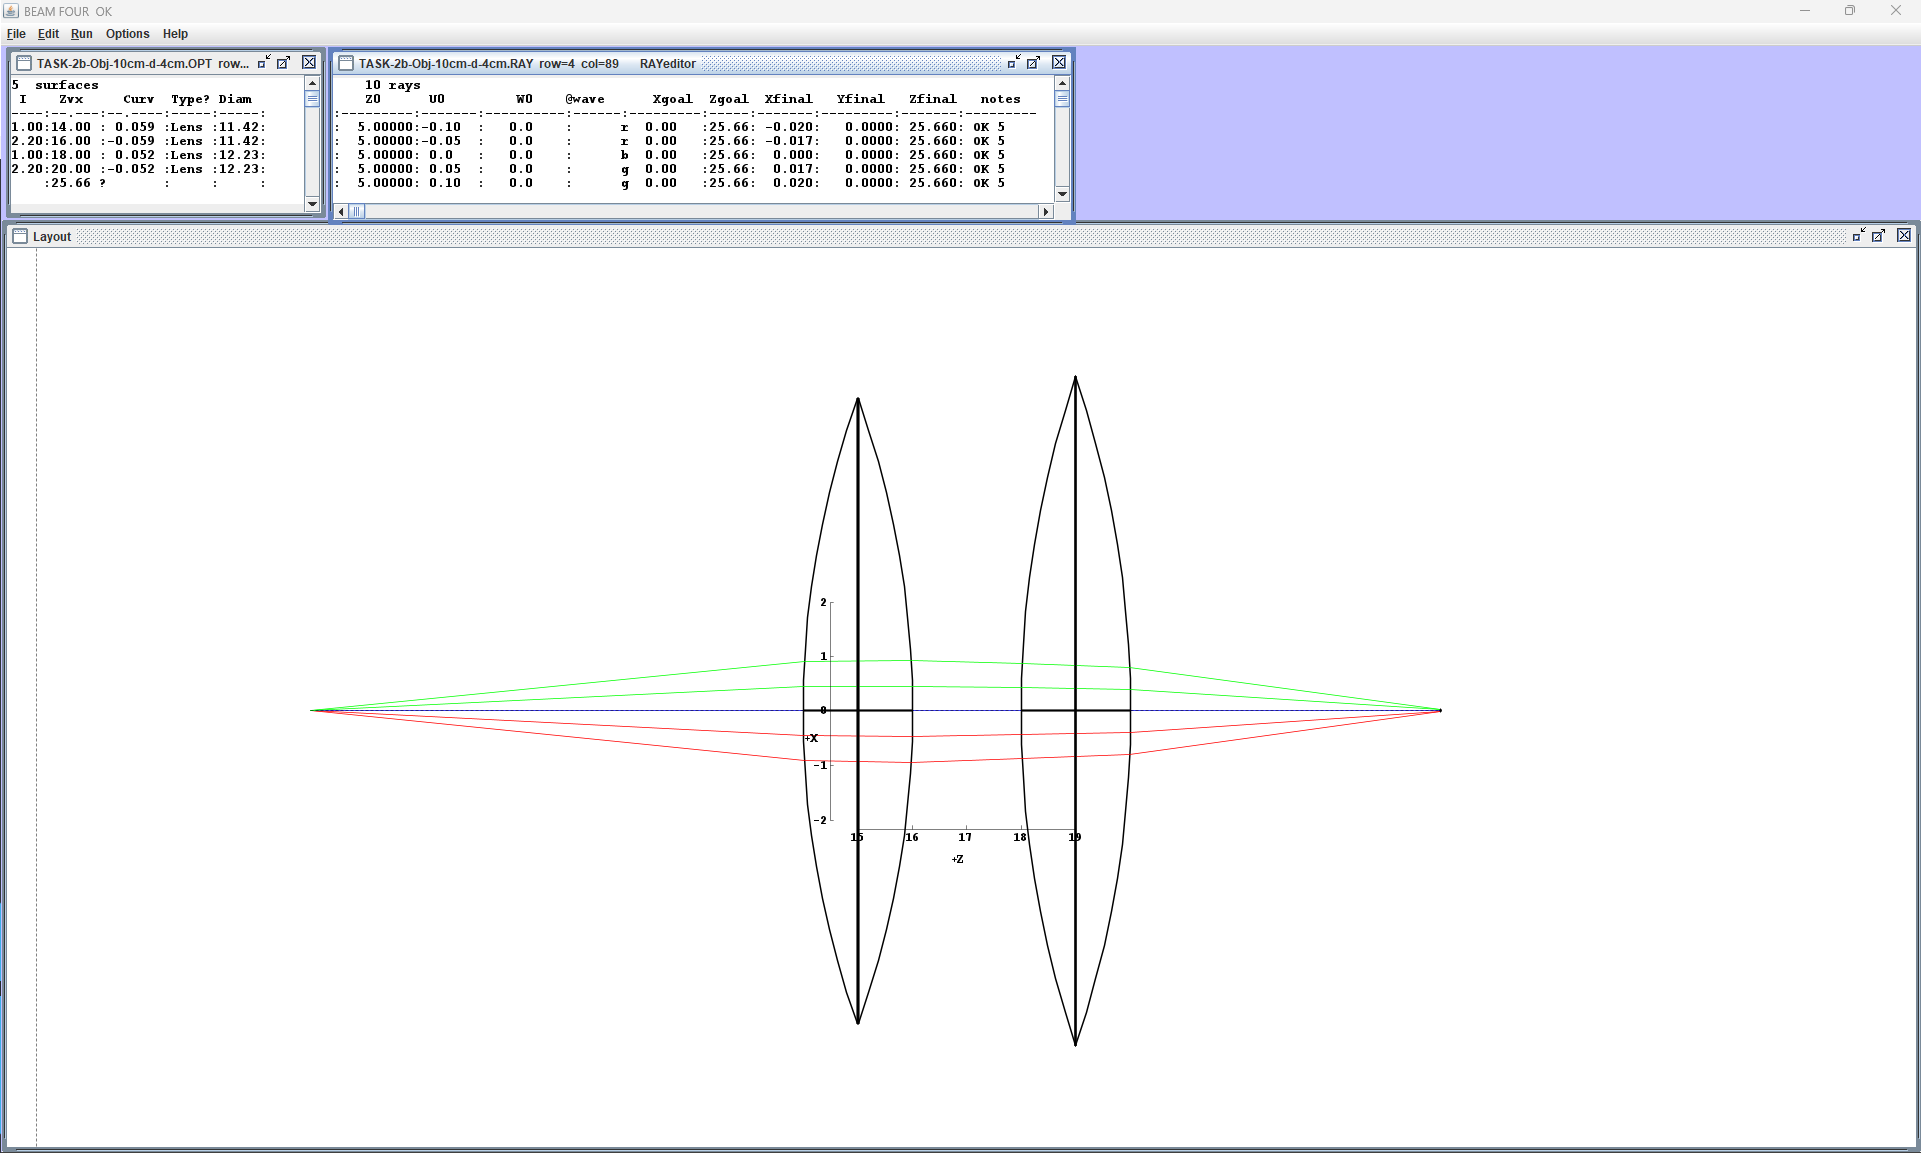
\includegraphics[width=0.75\linewidth]{Images/T2b-obj-10cm-d-4cm-Full-Window.png}
			\caption{\centering\footnotesize The beams traveling from left to right, with the relevant system parameters and final values shown.}
			\label{fig:t2b}
		\end{figure}
		
		
\end{document}
